\documentclass[a4paper,12pt]{report}

\usepackage{cmap}
\usepackage[T2A]{fontenc}
\usepackage[utf8]{inputenc}
\usepackage[english,russian]{babel}
\usepackage{listings}
\usepackage{amsmath}
\usepackage{amsfonts}
\usepackage{float}
\usepackage{csquotes}
\usepackage{hyphenat}

% \usepackage{titlesec}
% \newcommand{\sectionbreak}{\clearpage}

\usepackage{graphicx}
\graphicspath{ {./images/} }

\usepackage{xcolor}
% \usepackage{courier}

\usepackage[
    backend=biber,
    style=alphabetic,
    sorting=ynt
]{biblatex}
\addbibresource{resources.bib}

\definecolor{buzzlightyear}{HTML}{8757A5}
\definecolor{grass}{HTML}{738D06}
\definecolor{sand}{HTML}{F18A2B}
\definecolor{comment}{HTML}{8E908B}

\lstdefinestyle{habrstyle}{
    backgroundcolor=\color{white},   
    commentstyle=\color{comment},
    keywordstyle=\bfseries\color{buzzlightyear},
    numberstyle=\tiny\color{comment},
    stringstyle=\color{grass},
    basicstyle=\ttfamily\footnotesize,
    breakatwhitespace=false,         
    breaklines=true,                 
    captionpos=b,                    
    keepspaces=true,                 
    numbers=left,                    
    numbersep=5pt,                  
    showspaces=false,                
    showstringspaces=false,
    showtabs=false,                  
    tabsize=4
}

\lstset{style=habrstyle}

\author{Луняк Николай}
\title{Лабораторная работа 8}
\date{\today}

\begin{document}
    \maketitle
    \tableofcontents
    \listoffigures
    \lstlistoflistings
    
    \chapter{Запуск \texttt{chap08.ipynb}}
    
    При увеличении \texttt{std} без увеличения \texttt{M} можно наблюдать, что наши \textquote{скачки} снова вернулись, как если бы мы взяли Boxcar-фильтр на \texttt{M} элементов. Действительно, при большом значении \texttt{std} нормальное распределение растягивается в time domain, сжимая при этом нормальное распределение, которое соответствует ему в frequency domain, делая его все более и более похожим на Boxcar-фильтр.
    
    \chapter{Исследование DFT нормального распределения}
    
    Сначала, как всегда, импорты.
    
\begin{lstlisting}[language=Python,caption=Импорты]
from thinkdsp import Signal, Sinusoid, SquareSignal, TriangleSignal, SawtoothSignal, ParabolicSignal
from thinkdsp import normalize, unbias, PI2, decorate
from thinkdsp import Chirp
from thinkdsp import read_wave
from thinkdsp import Spectrum, Wave, UncorrelatedGaussianNoise, Spectrogram
from thinkdsp import Noise

import numpy as np
import pandas as pd

from matplotlib import pyplot as plt

import thinkstats2

from scipy.stats import linregress

import scipy
import scipy.fftpack

import scipy.signal

from ipywidgets import interact, interactive, fixed
import ipywidgets as widgets

loglog = dict(xscale='log', yscale='log')

PI2 = np.pi * 2
\end{lstlisting}

    Теперь будем строить рядом нормальное распределение (сигнал \textquote{во времени}) и его DFT. DFT будет как будто бы разрезано и разнесено в разные стороны, что решается при помощи \sloppy{\texttt{np.roll()}}.
    
\begin{lstlisting}[language=Python,caption=Импорты]
def plot_gaussian(std):
    M = 32
    gaussian = scipy.signal.gaussian(M=M, std=std)
    gaussian /= sum(gaussian)
    
    plt.subplot(1, 2, 1)
    plt.plot(gaussian)
    decorate(xlabel='Time')

    fft_gaussian = np.fft.fft(gaussian)
    fft_rolled = np.roll(fft_gaussian, M//2)
    
    plt.subplot(1, 2, 2)
    plt.plot(np.abs(fft_rolled))
    decorate(xlabel='Frequency')
    plt.show()

slider = widgets.FloatSlider(min=0.1, max=10, value=2)
interact(plot_gaussian, std=slider)
\end{lstlisting}
    
    \begin{figure}[H]
        \centering
        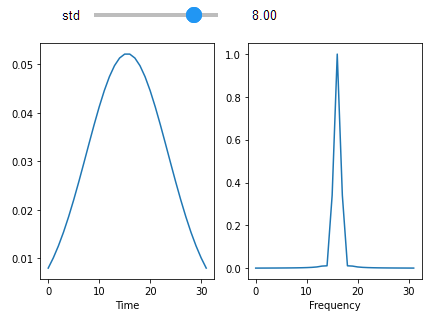
\includegraphics[width=0.75\textwidth]{images/ex2_comparison.png}
        \caption{Сравнение}
        \label{fig:ex2_comparison}
    \end{figure}
    
    Как я и писал в прошлом разделе, сужение одного \textquote{колокола} ведет к расширению другого.
    
    \chapter{Сравнение разных окон}
    
    В рамках данного пункта постараемся сравнить между собой разные окна, которые мы рассматривали в третьей лабораторной работе.
    
\begin{lstlisting}[language=Python,caption=Создание окон]
signal = SquareSignal(freq=440)
wave = signal.make_wave(duration=1.0, framerate=44100)

M = 15
std = 2.5

gaussian = scipy.signal.gaussian(M=M, std=std)   
bartlett = np.bartlett(M)
blackman = np.blackman(M)
hamming = np.hamming(M)
hanning = np.hanning(M)

windows = [blackman, gaussian, hanning, hamming]
names = ['blackman', 'gaussian', 'hanning', 'hamming']

for window in windows:
    window /= sum(window)
    
for window, name in zip(windows, names):
    plt.plot(window, label=name)

decorate(xlabel='Index')
\end{lstlisting}

    Нарисуем DFT каждого из них на одном графике.
    
\begin{lstlisting}[language=Python,caption=DFT]
def zero_pad(array, n):
    """Extends an array with zeros.

    array: NumPy array
    n: length of result

    returns: new NumPy array
    """
    res = np.zeros(n)
    res[:len(array)] = array
    return res

def plot_window_dfts(windows, names):
    for window, name in zip(windows, names):
        padded =  zero_pad(window, len(wave))
        dft_window = np.fft.rfft(padded)
        plt.plot(abs(dft_window), label=name)
        
plot_window_dfts(windows, names)
decorate(xlabel='Frequency (Hz)')
\end{lstlisting}

    \begin{figure}[H]
        \centering
        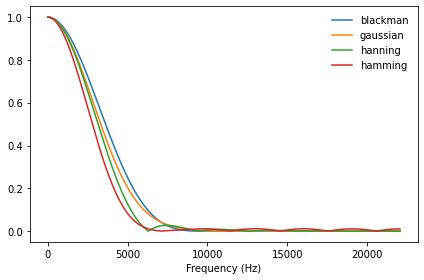
\includegraphics[width=0.75\textwidth]{images/ex3_linear.png}
        \caption{DFT}
        \label{fig:ex3_linear}
    \end{figure}

    Различия есть в отскоках, но их сложно заметить, поэтому отобразим то же самое в логарифмическом масштабе через 
    
\begin{lstlisting}[language=Python,caption=DFT в логарифмическом масштабе]
plot_window_dfts(windows, names)
decorate(xlabel='Frequency (Hz)', yscale='log')
\end{lstlisting}

    \begin{figure}[H]
        \centering
        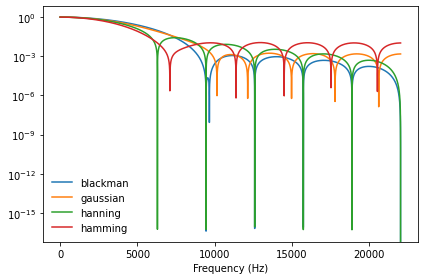
\includegraphics[width=0.75\textwidth]{images/ex3_log.png}
        \caption{DFT в логарифмическом масштабе}
        \label{fig:ex3_log}
    \end{figure}
    
    Среди всех самые \textquote{низкие} отскоки вышли у Хэннинга. При этом, он и Блэкмен продолжают уменьшаться, в то время как Хэмминг, несмотря на скачки, вроде как, держится на одном уровне (хотя поначалу он уменьшался быстрее всех остальных).    
    
    % \printbibliography
    
\end{document}
